\documentclass[12pt]{article}

\usepackage{amsmath}

\usepackage{graphicx}

\usepackage{hyperref}

\usepackage{graphicx}
\graphicspath{ {./images/} }


\usepackage[utf8]{inputenc}

\title{Operating System}
\author{Yuqiao Meng}
\date{2021–9–124}

\begin{document}

\maketitle

\newpage
\tableofcontents

\newpage

\section{Overview}

\subsection{What?}

What is an Operating System? What's its reponsibility?

\begin{itemize}
    \item A bunch of software and data residing somewhere in memory.
    \item The most privileged software in a computer. It  can do special things, like write to disk, talk over the network, control memory and CPU usage, etc
    \item Manages all system resources, including CPU, Memory, and I/O devices.
\end{itemize}

\subsection{Why?}
Why do we need an OS?
\begin{itemize}
    \item OS helps program to control hardwares.
    \item OS determines the way programs share resources.
    \item OS protects hardwares and programs from getting attacked.
    \item OS stores files persistently.
\end{itemize}
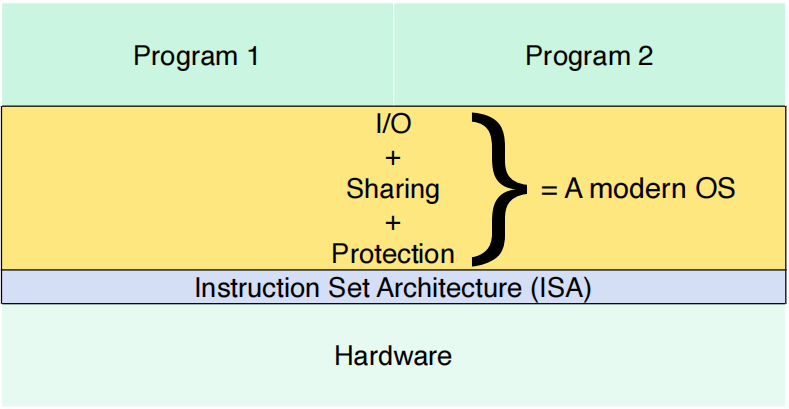
\includegraphics[width=1.0\textwidth]{WhyDoWeNeedOS.png}

\subsection{How}
\subsubsection{Virtulization}
\begin{itemize}
    \item Definition: OS takes a physical resource (such a sthe processor, or memory, or a disk) and transforms it into a more general, powerful, and easy-to-use virtual form of itself.
    \item Resource Virtulization \begin{itemize}
        \item Many(virtual)-to-one(physical): CPU Virtulization
        \item One-to-many: Disk Virtulization
        \item Many-to-many
    \end{itemize}
\end{itemize}
\subsubsection{How to invoke OS code?}
\begin{itemize}
    \item System calls: Function calls into the OS, that OS provides these calls to run programs, access memory and devices, and other related actions.
    \item Exceptions: CPU will raise an exception to the OS when the running program do something wrong
    \item Interrupts: Hardwares send interrupts to invoke OS
    \item Kernel Threads: Programs run in the kernel context, executing kernel level functions.
\end{itemize}
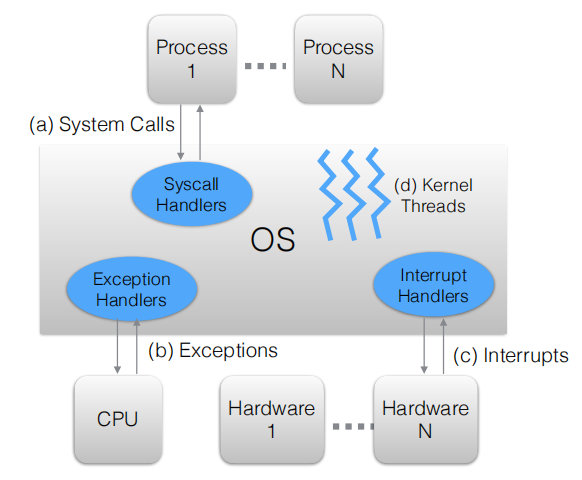
\includegraphics[width=0.8\textwidth]{FourWaysToInvokeOS.png}

\subsection{Interface}
\subsubsection{Explaination}
\begin{itemize}
    \item Instruction Set Architecture(ISA): the language CPU understand
    \item User ISA: ISA that any program can execute, it's accessible for all programs, doesn't need the service of operating system
    \item System ISA: ISA that only operating system is allowed to execute.
    \item Application Binary Interface(ABI): the combination of syscalls and User ISA(3, 7), it's the view of the world, seen by programs.
    \item Application Programmers' Interface(API): the combination of libraries and User ISA(2, 7), it's the tools programmer use to write codes.
\end{itemize}
\subsubsection{Interfaces in a Computer System}
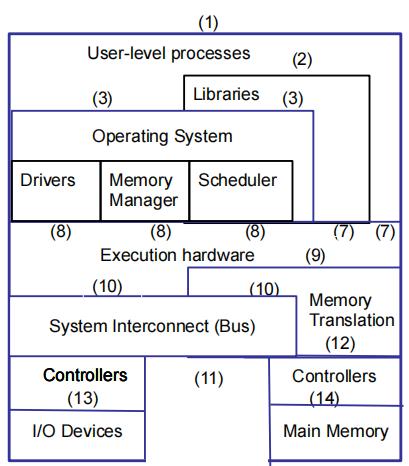
\includegraphics[width=0.6\textwidth]{InterfacesInComputerSystem.png}
\begin{itemize}
    \item User ISA: 7
    \item System ISA: 8
    \item Syscalls: 3
    \item Application Binary Interface: 3, 7
    \item Application Programmers' Interface: 2, 7
\end{itemize}

\subsection{History}
\begin{itemize}
    \item First Computer: Atanasoff–Berry computer, or ABC.
    \item First OS: GM-NAA I/O, produced in 1956 by General Motors' Research division for its IBM 704.
    \item First language: Plankalkül, developed by Konrad Zuse for the Z3 between 1943 and 1945.
    \item First programmer: Ada Lovelace
\end{itemize}

\section{Processes}
\subsection{Process}
\subsubsection{What?}
What is a process?
\begin{itemize}
    \item A process is a program in execution. A program is a set of instructions somewhere (like the disk).
    \item Once created, a process continuously does the following: \begin{itemize}
        \item {\bfseries Fetches} an instruction from memory. 
        \item {\bfseries Decodes} it. i.e., figures out which instruction this is. 
        \item {\bfseries Executes} it. it does the thing that it is supposed to do, like add two numbers together, access memory, check a condition, jump to a function, and so forth.
    \end{itemize}
\end{itemize}

\subsubsection{Process versus Program}
How is a process different from a program?
\begin{itemize}
    \item Program: A passive entity stored in the disk, has static code and static data.
    \item Process: Actively executing code and the associated static and dynamic data.
    \item Program is just one component of a process.
    \item There can be multiple process instances of the same program
\end{itemize}

\subsubsection{Constitution}
\begin{itemize}
    \item Memory space
    \item Procedure call stack
    \item Registers and counters
    \item Open files, connections
    \item And more.
\end{itemize}

\subsubsection{Memory layout}
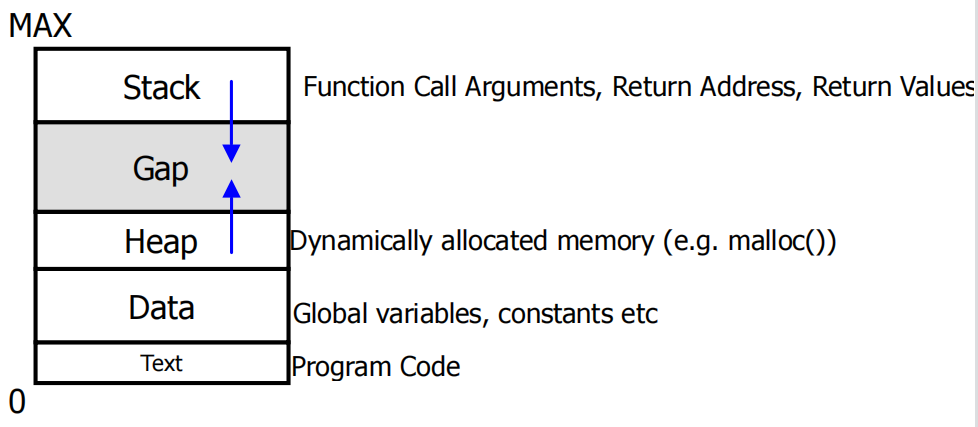
\includegraphics[width=1.0\textwidth]{ProcessMemoryLayout.png}
In this picture, Stack and Heap grow toward each other, that's because every process has a limited amount of space, thus let heap and stack grow toward each other from two direction can make the best use of space.

\subsection{System calls}
\begin{itemize}
    \item fork(): create new process. {\bfseries called once but return twice}. Usage: \begin{itemize}
        \item User runs a program at command line
        \item OS creates a process to provide a service: Check the directory /etc/init.d/ on Linux for scripts that start off different services at boot time.
        \item One process starts another process: For example in servers
    \end{itemize}
    \item exec(): execute a file. {\bfseries replaces the process’ memory with a new program image. All I/O descriptors open before exec stay open after exec}.
    \item wait()/waitpid(): wait for child process.
    \item exit(): terminate a process
\end{itemize}

\subsection{Lifecycle}
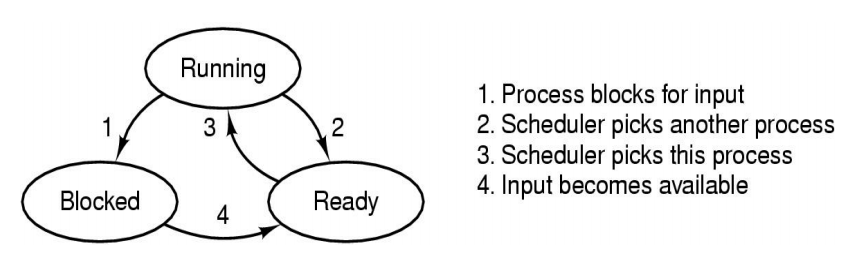
\includegraphics[width=1.0\textwidth]{ProcessLifecycle.png}
\begin{itemize}
    \item Ready (runnable; temporarily stopped to let another process run)\begin{itemize}
        \item Process is ready to execute, but not yet executing 
        \item Its waiting in the scheduling queue for the CPU scheduler to pick it up. 
    \end{itemize}
    \item Running:  (actually using the CPU at that instant) 
    \item Blocked (unable to run until some external event happens).\begin{itemize}
        \item Process is waiting (sleeping) for some event to occur. 
        \item Once the event occurs, process will be woken up, and placed on the scheduling queue
    \end{itemize}
\end{itemize}

\begin{enumerate}
    \item Running {$\to$} Blocked: Occurs when the operating system discovers that a process cannot continue right now.
    \item Running {$\to$} Ready: Occurs when the scheduler decides that the running process has run long enough and it is time to let another process have some CPU time.
    \item Ready {$\to$} Running: Occurs when all the other processes have had their fair share and it is time for the first process to get the CPU to run again.
    \item Blocked {$\to$} Ready: Occurs when the external event for which a process was waiting (such as the arrival of some input) happens
\end{enumerate}


\subsection{Special Process}
\begin{itemize}
    \item Orphan process \begin{itemize}
        \item When a parent process dies, child process becomes an orphan process
        \item The init process (pid = 1) becomes the parent of the orphan processes
    \end{itemize}
    \item Zombie process \begin{itemize}
        \item When a child dies, a SIGCHLD signal is sent to the OS, If parent doesn’t wait()on the child, and child exit()s, it becomes a zombie.
        \item Zombies hang around till parent calls wait() or waitpid().
        \item Zombies take up no system resources, it's just a integer status kept in the OS.
        \item Ways to prevent a child process from becoming a zombie: \begin{itemize}
            \item Parent call wait()/waitpid() before child process exit()
            \item Child parent sleep() before exit() until parent process give it a message.
        \end{itemize}
    \end{itemize}
\end{itemize}

\subsection{Cold-start Penalty}
\subsection{Context Switch}

\section{Inter-Process Communication}
\subsection{Overview}
Inter-Process Communication mechanisms
\begin{itemize}
    \item Pipe: 
    \item Signals: Event notification from one process to another
    \item Shared momery: Common piece of read/write memory, needs authorization for access
    \item Parent-child: Command-line arguments, including waitpid(), wait(), exit()
    \item Reading/modifying common files
    \item Semaphores: Locking and event signaling mechanism between processes
    \item Sockets: Not just across the network, but also between processes
\end{itemize}

\subsection{Pipe}

\end{document}